\chapter{The Pricing Problem}
\label{sec:the-pricing-problem}

\mytodo{These introductory paragraphs are either written like shit, duplicated or out-of-date. Please fix them.}

While the ESPPRC can be studied as a separate standalone problem,
here we are instead interested in the contributions that it can
provide in the context of pricing for the CVRP.

In this chapter we will cover in more details the pricing sub-problem
induced from the column generation scheme in BPC frameworks.
We've already the pricing problem in sections ....
In this chapter we will provide mathematical descriptions
of this problem by exploiting Integer Programming (IP).

While there may be multiple resources in play with different semantics
(time, capacity, gasoline, etc)
in the ESPPRC problem,
in this thesis we are mainly focused in ESPPRC subject to the single resource: the vehicle capacity.
Monotonic consumption of the resources.
Sometimes the ESPPRC subject to only the capacity constraint is called the Elementary Shortest
Path Problem with Capacity Constraints (ESPPCC).
It is however important to acknowledge that in the general case the ESPPRC allows for modeling
the pricing problems of many VRP variants such as the VRPTW, where also the "time resource"
plays a critical role.

Label-correcting dynamic programming approaches
dominate as the main approach to solve the (E)SPPRC in the context of pricing,
see \cite{desrochers1992, feillet2004, righini2004, righini2006, boland2006, righini2008, pugliese2010, baldacci2011, lozano2013, lozano2016, sadykov2021bucket}.
The proposed algorithm is a natural extension of the Bellman–Ford algorithm \parencite{bellman1958, fordjr1956},
a common algorithm present in the "toolbelt" of all operations research practitioners,
which computes shortest paths from a source vertex to all other vertices,
by taking also in consideration additional path constraints.
To the best of our knowledge,
branch-and-cut approaches for tackling the (E)SPPRC have been barely covered.
The few branch-and-cut contributions that we are aware of are:
\textcite{jepsen2008branchandcut} for the ESPPCC,
\textcite{jepsen2011,jepsen2014} to the CPTP (a special case of ESPPCC),
\textcite{taccari2016} for the non-resource constrained ESPP.
Branch-and-cut solutions for the general ESPPRC have not been covered,
and this is probably to the inherent two difficulties in modeling time windows constraints within IP formulations.
First, the IP formulation would require to model a directed network thus leading to a doubled size model.
Second, the delicate usage of big-M constraints are required to model resource constraints
that have bounds at the edge or node level (such as time-windows constraints).
Unfortunately, big-M constraints are inherently computationally unstable \parencite{jepsen2008branchandcut}.

\section{The Elementary Shortest Path Problem with Capacity Constraints}
\label{sec:the-elementary-shortest-path-problem-with-resource-constraints}

This section is dedicated to the discussion of the
Elementary Shortest Path Problem with Capacity Constraints (ESPPCC)
in the context of pricing for the CVRP.
While we have already glimpsed at the general ESPPRC case of this problem in
\cref{sec:column-generation-and-pricing-problem,sec:intro-solving-the-pricing-problem},
we've never provided a formal description of the mathematical model.
In this section we consider the basic version of the ESPPCC,
i.e. non-robust inequalities at the RMP level are not considered.
In case non-robust inequalities are employed,
ESPPCC does not suffice in modeling the pricing problem.
A slight variation of the ESPPCC characterized by additional constraints
becomes mandatory to ensure correctness of the column generation approach.

The ESPPCC asks for the determination of the shortest path on a weighted network
between two vertices $s, t$
subject to a single global resource restriction characterized
by the amount of goods available for serving.
In the ESPPCC problem,
the elementarity condition imposes that no optimal path may
cover the same vertices two or more times.
The ESPPCC's underlying network may in the general case,
contain negative cost cycles.
The presence of negative cost cycles makes solving such problem NP-hard \parencite{dror1994}.
A dynamic programming algorithm
to tackle the elementary version of the problem
was proposed in \textcite{feillet2004}.
However, in the context of pricing, the problem has been traditionally relaxed into a SPPRC.
The SPPRC,
contrary to the elementarity version,
can be solved in pseudo-polynomial time with a much faster dynamic programming algorithm \parencite{desrochers1992}.
Unfortunately,
relaxing the elementarity condition leads to slower column generation and worsening of dual bounds,
see previous discussion in \cref{sec:intro-solving-the-pricing-problem}.

\medskip

In the case that the ESPPCC's weighted network contains no non-negative
cost cycles, the elementarity condition maybe safely dropped \parencite{beasley1989}.
A sufficient but not-necessary condition is when the reduced cost variables
are all positive: $\bar{c}_{ij} \ge 0 \quad \forall i, j \in V_0 \cup \Set*{s, t}$.
In such case, an optimal solution of the associated non-elementary SPPRC problem
is an optimal solution to the original elementary version of the problem \parencite{beasley1989}.
The associated SPPRC can be solved efficiently in pseudo-polynomial time.
Initial contributions for tackling the ESPCC exploited this property.
The resource consumption constraint was relaxed through a Lagrangean relaxation
approach.
Through the usage of a branch-and-bound scheme and an off-the-shelf
standard shortest path algorithm, e.g. Dijkstra \parencite{sniedovich2006dijkstra},
they obtained feasible dual solutions over strictly positive weighted networks.
See the contributions of
\textcite{beasley1989, dumitrescu2003improved, carlyle2008, muhandiramge2009simultaneous},
just to name a few.
But as pointed out in \textcite{righini2004},
Lagrangian relaxation is effective only when the dualized variables
are positive for a good portion of the Lagrange multipliers search space,
which limit the effectiveness of these approaches in the context of pricing.

\subsection{Integer Programming Formulation}
\label{sec:espprc-integer-programming-formulation}

While \textcite{jepsen2008branchandcut} provides
an \textbf{undirected} symmetric network based formulation for the ESPPCC,
in our presentation we have preferred instead to re-adjust the more-general
\textbf{directed} symmetric network based ESPPRC formulation
provided in the works of \textcite{beasley1989, toth2002, toth2014}.
For this reason we need to readjust/extend the
mathematical notation that was originally provided for the undirected CVRP in \cref{sec:intro-cvrp-mathematical-notation}.

\medskip

The ESPPCC network is characterized by $N^\prime = N_0 + 2$ nodes,
where $N_0$, denotes the total number of customers in the original CVRP problem.
Two additional vertices $s = 0, t = N^\prime - 1$ are used to represent respectively the source and sink vertices.
These two together model a dissection of the depot node.
All the customers are edge-connected in both directions with one another.
Similarly, the source and sink vertex do not share direct connections together.

More formally, the ESPPCC is defined over a directed symmetric network
$G^\prime = \Tuple*{V^\prime, A^\prime}$,
where $V^\prime = V_0 \cup \Set*{s, t}$ denotes the set of vertices and $A^\prime$ the set of arcs.
The vertices $s = 0,\ t = N^\prime - 1$ denote respectively the source and sink versions of the depot node.
The vertex set $V^\prime$ has size $|V^\prime| = N^\prime = N_0 + 2$.
The edges set $A^\prime$ can be expressed as:
\begin{equation}
	\begin{aligned}
		A^\prime = \  & \Set*{\Tuple*{i, j} \mid i, j \in V_0,\ i \ne j} \\
		              & \cup \Set*{\Tuple*{s, i} \mid i \in V_0}         \\
		              & \cup \Set*{\Tuple*{i, t} \mid i \in V_0}.
	\end{aligned}
\end{equation}
The edge set $A^\prime$ has size $|A^\prime| = N^\prime(N^\prime - 1) + 2(N^\prime - 1)$.
In accordance to the CVRP problem,
we associate a resource consumption, or vertex demand,
to each node of the network: $q_i \quad \forall i \in V^\prime$.
The resource consumption semantics associated with each customer
$i \in V_0$ remains unaltered  from the CVRP, while for the source and sink vertices
we respectively fix $q_{s} = q_{t} = 0$.
We formally define $\deltaplus(S) = \Set*{(i, j) \in A^\prime \mid i \in S, j \notin S}$
to denote the out-arcs crossing the set $S \subset V^\prime$.
Likewise, we define $\deltaminus(S) = \Set*{(i, j) \in A^\prime \mid i \notin S, j \in S}$
to denote the in-arcs crossing the set $S \subset V^\prime$.
For brevity’s sake,
we also define $\deltaplus(i) = \deltaplus(\Set*{i})$, $\deltaminus(i) = \deltaminus(\Set*{i})$
to denote respectively the singleton version of the in and out arcs for vertices $i \in V^\prime$.
Note that the following conditions hold:
$\deltaplus(s) = V_0,\ \deltaminus(t) = V_0,\ \deltaminus(s) = \emptyset,\ \deltaplus(t) = \emptyset$.
We also define $A^\prime(S) = \Set*{\Tuple*{i, j} \in A^\prime \mid i, j \in S}$
to denote the set of arcs having both end points in set $S \subseteq V^\prime$.

As it was done in \cref{sec:column-generation-and-pricing-problem},
for each directed arc we associate a weight
$\bar{c}_{ij} \in \R \quad \forall \Tuple*{i, j} \in A^\prime$.
The weight $\bar{c}_{ij}$ represents the reduced cost of an arc $\Tuple*{i, j} \in A^\prime$.
Its definition is linked to the dual variables $\pi \in \R^N$ associated to
the RMP's constraints of \cref{eq:mp-K-routes,eq:mp-customers-visited-by-exactly-one-route}
through the following relationship:
\begin{equation}
	\bar{c}_{ij} = \begin{cases}
		c_{ij} - \frac{\pi_i + \pi_j}{2} & \quad \forall i, j \in V_0 \\
		c_{si} - \frac{\pi_0 + \pi_j}{2} & \quad \forall j \in V_0    \\
		c_{it} - \frac{\pi_i + \pi_0}{2} & \quad \forall i \in V_0    \\
		\infty                           & \quad \texttt{otherwise}
	\end{cases}
\end{equation}
Additional usage of robust inequalities (cuts or branching) manifest
additional negative term contributions, through additional dual variables,
directly to the reduced arc cost $\bar{c}_{ij}$.
See previous discussion in \cref{sec:intro-branching-and-cut-generation-within-bap-frameworks}.

A feasible path solution to the ESPPCC is a sequence $p = \Tuple*{p_0, p_1, \dots, p_s, p_{u+1}}$
with $p_0 = s, \ p_{u + 1} = t$
in which $\Set*{p_1, \dots, p_u} \subseteq V_0$ customers are visited.
Observe that there's no restriction in which customers need to be necessarily covered
by the path $p$.
Due to the elementarity condition, the path $p$ can cover a vertex at most once.
The path's resource consumption $q_p = q(p) = \sum_{j=0}^{u} q_{p_j}$
satisfies $q(p) \le Q$.
The optimal path $p^\star$ minimizes the overall path's reduced cost
$\bar{c}(p) = \sum_{i=0}^{u} \bar{c}_{p_i,p_{i+1}}$ across all
possible feasible choices for $p$.
Note that, regardless we have decided to model
the dual variables contributions $\pi \in \R^N$
at the arc level instead at the vertex level,
the path reduced cost still sums to:
$\bar{c}(p) = \sum_{i=0}^{u} c_{p_i,p_{i+1}} - \sum_{i=0}^{u} \pi_{p_i} = c(p) - \sum_{i=0}^{u} \pi_{p_i}$.
Therefore, $\pi_i \in R,\ i \in V_0$ can be interpreted as the
gained profit obtained in serving customer $i \in V_0$.
Similarly,
$\pi_0 \in R$ can be interpreted as an additional constant term
biasing the reduced cost of a feasible route $p$.

\medskip

We are now ready to provide a ESPPCC formal description through an Integer Programme (IP).
Let $x_{ij} \in \Set*{0, 1} \quad \Tuple*{i, j} \in A^\prime$ be a new set of binary variables:
$x_{ij} = 1$ if arc $\Tuple*{i, j} \in A^\prime$ is picked by the optimal path.
We can provide a formal mathematical formulation of the ESPPCC as an Integer Programme (IP):
\begin{align}
	\min_{x} \quad z_\mt{ESPPCC}(x) & =  \sum_{(i, j) \in A^\prime} \bar{c}_{ij} x_{ij}                                                     \label{eq:espprc-obj-function}                                                                \\
	                                & \sum_{i \in V_0} \frac{q_i}{2} \Expr*{ \ExprESPPIngoingEdges{i} + \ExprESPPOutgoingEdges{i} }  \le Q  \label{eq:espprc-resource-upper-bound-constraint}                                             \\
	                                & \ExprESPPIngoingEdges{i} = \ExprESPPOutgoingEdges{i}                                                  \qquad \forall i \in V_0          \label{eq:espprc-flow-conservation-constraint-customers}    \\
	                                & \ExprESPPOutgoingEdges[i]{s} = 1                                                                      \label{eq:espprc-source-emitting-flow}                                                        \\
	                                & \ExprESPPIngoingEdges[i]{t} = 1                                                                       \label{eq-espprc-sink-consuming-flow}                                                         \\
	                                & \ExprESPPEdgesWithin[S] \le |S| - 1                                                                   \qquad \forall S \subseteq V_0 \cup \Set*{s, t},\ |S| \ge 2 \label{eq:espprc-sec-constraints} \\
	                                & x_{ij}                   \in \lbrace 0, 1 \rbrace                                                     \qquad \forall \Tuple*{i, j} \in A^\prime    \label{eq:espprc-x-mip-var-bounds},
\end{align}
where \labelcref{eq:espprc-obj-function} is the objective function to be minimized, i.e. the overall reduced cost of the path.
Constraint \labelcref{eq:espprc-resource-upper-bound-constraint} is the resource consumption upper bound.
Constraint \labelcref{eq:espprc-flow-conservation-constraint-customers} imposes a flow conservation for all vertices except for the source and the sink.
Observe that \cref{eq:espprc-flow-conservation-constraint-customers} does not impose
restriction on whether customer $i \in V_0$ needs to be necessarily covered by the path.
Constraints \labelcref{eq:espprc-source-emitting-flow}, \labelcref{eq-espprc-sink-consuming-flow}
respectively impose an out-flow and in-flow of $1$ for the source and sink vertices.
Constraints \labelcref{eq:espprc-sec-constraints} are the Subtour Elimination Constraints (SEC) and
have a two-fold effect.
First, they avoid the formation of spurious tours in unconnected regions of the network, such
as the situation depicted in \cref{fig:espprc-example-with-spurious-subtours}.
Second, they impose the elementarity condition, restricting paths from visiting multiple times
the same vertices, such as the situation depicted in \cref{fig:espprc-example-non-elementary-solution}.
Constraint \labelcref{eq:espprc-x-mip-var-bounds} imposes integrality
and forces each arc $\Tuple*{i, j} \in A^\prime$ to be traversed at most once.

Notice that, due to the flow conservation constraint and to the bounds on the binary varibles of
\cref{eq:espprc-flow-conservation-constraint-customers,eq:espprc-x-mip-var-bounds},
we have that the following equality holds:
\begin{equation}
	\ExprESPPIngoingEdges{i} + \ExprESPPOutgoingEdges{i} = \begin{cases}
		2 & \texttt{if } i \in p \\
		0 & \texttt{otherwise}
	\end{cases}
	\quad \forall i \in V_0.
\end{equation}
Regardless of a constant factor of $2$,
the quantity $\ExprESPPIngoingEdges{i} + \ExprESPPOutgoingEdges{i}$
can be used to determine the number of times a  customer $i \in V_0$ is visited.

The resource consumption constraint of \Cref{eq:espprc-resource-upper-bound-constraint} is
expressed at the vertex level.
Equivalently, it is possible to express the same constraint by considering the resource consumption
at the arc level:
\begin{equation}
	\label{eq:espprc-resource-upper-bound-constraint-arc-level}
	\sum_{\Tuple*{i, j} \in A^\prime} \frac{q_i + q_j}{2} x_{ij} \le Q.
\end{equation}
Due to the structure of the optimal path $p^\star$ the total resource consumption
will not change regardless of whether
\labelcref{eq:espprc-resource-upper-bound-constraint}
or \labelcref{eq:espprc-resource-upper-bound-constraint-arc-level}
is used.

\begin{figure}[ht]
	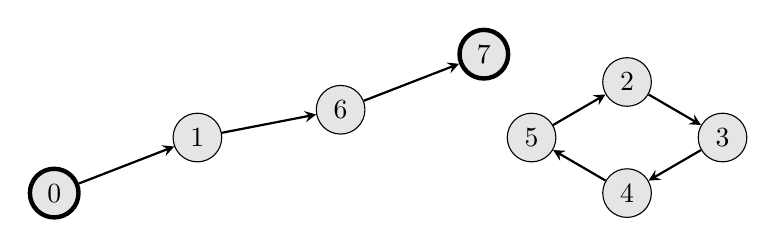
\begin{tikzpicture}[>=stealth, main/.style = {draw, circle, fill=black!10!white}]
		\centering

		\node[main, ultra thick] (0) at (0.1\textwidth,-20bp) {0};
		\node[main] (1) at (0.25\textwidth,0bp){1};
		\node[main] (6) at (0.4\textwidth,+10bp){6};
		\node[main, ultra thick] (7) at (0.55\textwidth,+30bp) {7};

		\node[main] (2) at (0.7\textwidth, +20bp){2};
		\node[main] (3) at (0.8\textwidth, -0bp) {3};
		\node[main] (4) at (0.7\textwidth, -20bp) {4};
		\node[main] (5) at (0.6\textwidth, -0bp) {5};

		\draw [->,thick] (0) -- (1);
		\draw [->,thick] (1) -- (6);
		\draw [->,thick] (6) -- (7);

		\draw [->,thick] (2) -- (3);
		\draw [->,thick] (3) -- (4);
		\draw [->,thick] (4) -- (5);
		\draw [->,thick] (5) -- (2);
	\end{tikzpicture}

	\centering
	\caption{
		An example of a path containing spurious unconnected sub-tours,
		over a network with $V^\prime = \Set*{0, \dots, 7},\ s = 0,\ t = 7$.
		The SEC inequalities of \cref{eq:espprc-sec-constraints} prohibit the depicted situation from occurring.
	}
	\label{fig:espprc-example-with-spurious-subtours}
\end{figure}

\begin{figure}[ht]
	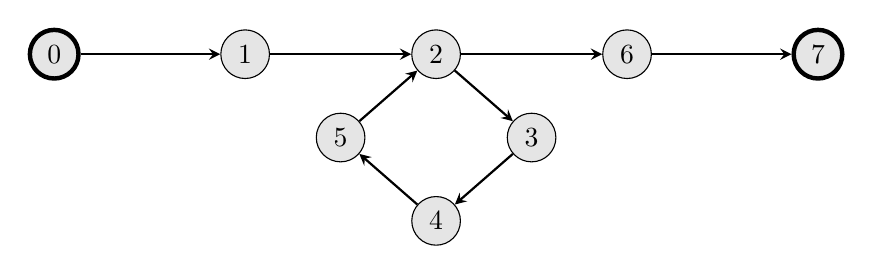
\begin{tikzpicture}[>=stealth, main/.style = {draw, circle, fill=black!10!white}]
		\centering

		\node[main, ultra thick] (0) at (0.1\textwidth,0bp) {0};
		\node[main] (1) at (0.3\textwidth,0bp){1};
		\node[main] (2) at (0.5\textwidth,0bp){2};
		\node[main] (3) at (0.6\textwidth,-30bp) {3};
		\node[main] (4) at (0.5\textwidth,-60bp) {4};
		\node[main] (5) at (0.4\textwidth,-30bp) {5};
		\node[main] (6) at (0.7\textwidth,0bp){6};
		\node[main, ultra thick] (7) at (0.9\textwidth,0bp) {7};

		\draw [->,thick] (0) -- (1);
		\draw [->,thick] (1) -- (2);
		\draw [->,thick] (2) -- (3);
		\draw [->,thick] (3) -- (4);
		\draw [->,thick] (4) -- (5);
		\draw [->,thick] (5) -- (2);
		\draw [->,thick] (2) -- (6);
		\draw [->,thick] (6) -- (7);
	\end{tikzpicture}

	\centering
	\caption{
		An example of a path not satisfying the elementarity constraints,
		over a network with $V^\prime = \Set*{0, \dots, 7},\ s = 0,\ t = 7$.
		The SEC inequalities of \cref{eq:espprc-sec-constraints} prohibit the depicted situation from occurring.
	}
	\label{fig:espprc-example-non-elementary-solution}
\end{figure}

As it is done in \textcite{beasley1989},
if one wishes to avoid the formation of spurious unconnected subtours
while relaxing the elementarity condition,
it can achieve so by substituting \cref{eq:espprc-sec-constraints} in favor
of a big-M constraint of the form:
\begin{equation}
	\label{eq:espprc-relaxed-elementarity}
	\ExprESPPEdgesWithin[S] \le M \ExprESPPEdgesCrossing[S] \quad \forall S \subseteq V_0 \cup \Set*{s}
\end{equation}
where $M \in \R_+$ denotes an arbitrary large positive constant.
\Cref{eq:espprc-relaxed-elementarity} avoids the situation depicted
in \cref{fig:espprc-example-with-spurious-subtours}
while permitting the situation depicted in \cref{fig:espprc-example-non-elementary-solution}.
Modeling the pricing as an SPPCC, can greatly reduce
the column generation running time, at the cost
of generating significantly weaker dual bound improvements.
Refer back to the discussion in \cref{sec:intro-solving-the-pricing-problem}
for more details.

Additional valid inequalities and a branch-and-cut framework
for the ESPPCC was provided in the work of \textcite{jepsen2008branchandcut}.
In this thesis we are mainly concerned with the CPTP in the context of pricing.
Therefore we will not spend more efforts in discussing the ESPPCC.

\section{The Capacitated Profitable Tour Problem}
\label{sec:the-capacitated-profitable-tour-problem}

The Capacitated Profitable Tour Problem, abbreviated as CPTP,
belongs to the group of the so-called travelling salesman
problems with profits (TSPP) (see \cite{feillet2005}),
and therefore presents many similarities with other very well known
problems such as:
(i) the Orienteering Problem (OP) \parencite{golden1987, laporte1990}
(ii) the Profitable Tour Problem (PTP) \parencite{dellamico1995},
(iii) the Prize Collecting Traveling Salesman Problem (PCTSP) \parencite{balas1989prize, balas1995prize},
(iv) the Capacitated m-Ring-Star Problem (CmRSP) \parencite{baldacci2007capacitated}.
See \textcite{letchford2013} for the Steiner extension of these problems.
The OP, an NP-hard problem \parencite{laporte1990}, asks for a route serving
a subset of customers with profits.
In OP, the route length is bounded in terms of number of vertices visited,
whereas in CPTP the route is bounded in terms of accumulated demand served
through the maximum available vehicle capacity.
Using the reduction to Hamiltonian circuit problem
employed to prove that the OP is NP-hard \parencite{laporte1990},
the same reasoning can be applied to conclude that CPTP is also NP-hard.
The CPTP has many roots in common with the OP, in fact,
the OP may be regarded as a special case of an edge-capacitated CPTP with unit demands.
Refer to \textcite{fischetti1998, gendreau1998} for contributions
exposing BAC frameworks and valid inequalities for the OP.
Many of such inequalities (but not all) are also valid for the CPTP \parencite{jepsen2014}.
We will introduce the CPTP in the context of pricing for the CVRP.
We will study the basic version of the CPTP,
i.e. we will not consider additional non-robust inequalities
at the RMP level that could change the structure of the problem.

In more details,
the CPTP is a combinatorial optimization delivery problem,
in which,
given as input a set of customers
defined over a fully connected undirected network, the goal resides in finding
a resource constrained elementary tour (or circuit) starting from a common point called the depot,
that minimizes the overall travel distance while maximizing
the profits associated in serving only a subset of the customers.
The elementarity constraint dictates that no vertex
can be visited twice or more, thus implying that the earnable profit
per customer is available only once.
The CPTP can also be described in simple words
as a single-truck ($k = 1$) (C)VRP where it is possible to serve only a small set of customers,
based on a profit value that is gained when serving occurs.
The CPTP shows up naturally as a sub-problem
in the column generation approach employed in solving many VRP variants.
It is an important special case of the
ESPPCC when the source and sink vertices are used to represent the same node.
Contrary to the traditional description of the ESPPCC,
the CPTP is easier to describe.
Its formulation can be provided on an undirected symmetric network,
reducing the total number of independent variables.
However, due to its narrower scope,
it is far less addressed in the literature compared to ESPPRC.

To the best of our knowledge, the few contributions studying the CPTP
in the context of pricing for the VRP can be found in \textcite{bixby1999, jepsen2011,jepsen2014}.
\textcite{jepsen2014} study the CPTP problem in the context of pricing for the VRP.
Their work originate from the initial efforts in \textcite{jepsen2008branchandcut},
were a branch-and-cut algorithm was applied to solve the ESPPCC.
Their work lays out a first foundational theory for further development
of the CPTP as an independent problem or as in the context of pricing.
Their work may serve in the future as a tutorial/survey/framework
for further development of branch-and-cut algorithms for the CPTP.
They propose a branch-and-cut framework for the CPTP,
along with a directed symmetric network IP formulation.
They adapt many valid inequalities from related problems,
introduce a new family of inequalities (rounded multistar inequalities)
discuss and implement their efficient separation,
and finally proposes an efficient heuristic for separating
the \textit{knapsack large multistar inequalities} \parencite{letchford2002}.
They study the competitiveness of their approach
along with the usefulness of the valid inequalities through a computational study.
Their results show that while a branch-and-cut framework based on CPTP may
not be competitive in solving the historical CVRP instances w.r.t. to dynamic programming in most cases,
it seemed to perform better when the number of nodes in the network increases,
or as the network weights were highly negative
and was slower on solutions where the objective value was very close to zero.
Unfortunately network with highly negative weights are usually
solved through heuristics,
while the bounding procedure of exact labeling algorithm is usually optimized
to cut off huge portions of the solution space in the latter case.
Nonetheless, \textcite{jepsen2014}
proved that such approach could provide a good complement
to the dynamic programming algorithms,
showing that there may be value in further developing
branch-and-cut frameworks for pricing in column generation schemes.

Attempting to solve the ESPPCC through branch-and-cut frameworks
have been lately attempted and evaluated in the works of \textcite{jepsen2008branchandcut}.
Along with empirical results,
these contributions provide IP mathematical models and additional valid inequalities.
\textcite{jepsen2008branchandcut} provides an IP formulation described over and undirected network.

The presentation of this section, along with the implementation of \cref{sec:implementation-chapter}
owes a lot to the efforts of \textcite{jepsen2014}.

\subsection{Integer Programming formulation}
\label{sec:cptp-integer-programming-formulation}

Our CPTP description follows closely the formulation provided in \textcite{jepsen2014}.
To describe the formulation
we will continue to use the mathematical notation introduced in \cref{sec:intro-cvrp-mathematical-notation}
for the CVRP and extend it.

Let $p_i \in \R,\ p \ge 0$ denote the profit associated in visiting a vertex $i \in V$.
The profit function is directly linked to the dual variables $\pi \in \R^N$ associated to
the RMP's constraints of \cref{eq:mp-K-routes,eq:mp-customers-visited-by-exactly-one-route}.
Namely, $p_i = \pi_i \quad \forall i \in V$.

Let $x_{e}$, $y_{i} \in \Set*{0, 1}$ be two sets of binary variables which respectively
model whether an edge $e \in E$ or vertex $i \in V$ is covered by the optimal CPTP route.
We can provide a formal mathematical description of the CPTP through an Integer Programme (IP) formulation:
\begin{align}
	\min_{x,y} \quad z_\mt{CPTP}(x, y) & = \ExprCptpObjValDef                     & \label{eq:cptp-obj-function}                                                                          \\
	                                   & y_0 = 1                                  & \label{eq:cptp-depot-part-of-tour-constraint}                                                         \\
	                                   & \ExprCptpDemandSum  \le Q                & \label{eq:cptp-resource-upper-bound-constraint}                                                       \\
	                                   & \ExprCptpEdgesIncident{i}  = 2 y_i       & \quad \forall i \in V         \label{eq:cptp-flow-conservation-constraint}                            \\
	                                   & \ExprCptpFlowExiting{S} \ge 2 y_{i}      & \quad \forall i \in S,\ \forall S \subseteq V_0,\ \SetSize*{S} \ge 2 \label{eq:cptp-gsec-constraints} \\
	                                   & x_{e}                   \in \Set*{0, 1}  & \quad \forall e \in E               \label{eq:cptp-x-mip-var-bounds}                                  \\
	                                   & y_{i}                    \in \Set*{0, 1} & \quad \forall i \in V             \label{eq:cptp-y-mip-var-bounds}
\end{align}
where \labelcref{eq:cptp-obj-function} is the objective function to be minimized, i.e. the cost
accounting for the total travel distance and the profit in serving a subset of the vertices.
Constraint \labelcref{eq:cptp-depot-part-of-tour-constraint} ensures that the depot is always covered by the optimal route.
Constraint \labelcref{eq:cptp-resource-upper-bound-constraint} is the resource consumption upper bound.
Constraint \labelcref{eq:cptp-flow-conservation-constraint} has a twofold effect.
First, it functions as a form of directed flow conservation.
Second, it binds the $x,\ y$ sets of variables together;
namely, it ensures that the if a vertex $i \in V$ is covered by an optimal route ($y_i = 1$)
then the number of incident edges in that node sums to $2$, otherwise to $0$.
Constraint \labelcref{eq:cptp-gsec-constraints}
are the so-called Generalized Subtour Elimination Constraints (GSECs),
which avoid the formation of spurious tours in unconnected regions of the network.
There is an exponential number of GSECs,
therefore for performance reasons,
these constraints cannot be inserted statically in a MIP solver,
and must instead be separated exactly at least for integral solutions.
Constraints \labelcref{eq:cptp-x-mip-var-bounds,eq:cptp-y-mip-var-bounds} respectively
impose bounds and integrality condition
on the number of traversal for edges $e \in E$ and vertices $i \in V$.
The IP model consists of $\frac{N^2 + N}{2}$ number of binary variables and an exponential number of constraints.
If we ignore the GSECs and variable bounds, the IP model owns a total of $N + 2$ constraints.
Constraints \labelcref{eq:cptp-gsec-constraints}
can also be rewritten in a different form \parencite{wolsey2020integer}:
\begin{equation}
	\label{eq:cptp-gsec-constraints-v2}
	\sum\limits_{e \in E(S)} x_e \le \sum\limits_{i \in S \setminus \Set*{j}} y_i \quad \forall j \in S,\ \forall S \subseteq V_0,\ |S| \ge 2.
\end{equation}
Equivalently,
the \cref{eq:cptp-resource-upper-bound-constraint}
can be defined at the edge level:
\begin{equation}
	\sum_{e = \Set*{i, j} \in E} \frac{q_i + q_j}{2} x_e \le Q
\end{equation}

Note that model
\labelcref{eq:cptp-obj-function,eq:cptp-depot-part-of-tour-constraint,eq:cptp-resource-upper-bound-constraint,eq:cptp-flow-conservation-constraint,eq:cptp-gsec-constraints,eq:cptp-x-mip-var-bounds,eq:cptp-y-mip-var-bounds}
does not permit for single-customer routes.
Instead of modifying the formulation to allow for this edge case,
it may be simpler to leave the model unchanged.
By employing a brute-force algorithm in $\Theta(N)$ time we can scan for improving single-customer solutions.
After the resolution of the IP model,
we check for improving single-customer solutions and,
if any exist,
we update the incumbent.

\section{Additional Valid Inequalities}
\label{sec:cptp-additional-valid-inequalities}

In this section we present additional valid inequalities for the CPTP problem.
While these additional inequalities are not strictly necessary
to ensure the correctness of the optimal solution,
when embedded inside an efficient branch-and-cut framework through efficient separation techniques,
can massively strengthen the linear relaxation and thus speed up the resolution process.

The inequalities that we present follow closely the presentation provided in \textcite{jepsen2014}.
Our presentation is not meant to be inclusive of every valid inequalities for the CPTP.
Instead, we will concentrate on the presentation of the most important ones
that we've considered in the final implementation of our branch-and-cut pricer.
Presentation of additional inequalities for the CPTP problem can be found in \textcite{jepsen2014}.

As pointed out in \textcite{jepsen2014},
RCIs seem to be frequently separable during the running time of the branch-and-cut procedure.
Suggesting that their usage, may likely lead to a speed-up in the resolution process
compared to the running time cost for their separation.

As pointed out in \textcite{jepsen2014},
GLMs seem to be frequently separable during the running time of the branch-and-cut procedure.
Suggesting that their usage, may likely lead to a speed-up in the resolution process
compared to the running time cost for their separation.
meaning that their usage is likely to speed up the resolution process.

\subsection{Rounded Capacity Constraints (RCC)}
\label{sec:cptp-rcc}

The Rounded Capacity Constraints, RCC for short, were first presented
for the CVRP  in \textcite{laporte1983}
and were already presented in \cref{sec:intro-cvrp-two-index-flow-formulation}.

Recall that $q(S) = \sum_{i \in S} q_i$ represents
the total demand in serving all vertices in set $S \subseteq V$.
The RCC constraints they function as a capacity constraint
by imposing that any customer set $S \subseteq V_0$ is crossed by a number of edges
not smaller by the number of trucks that would be necessary to serve all customers in $S \subseteq V_0$.
The RCC can be extended to the CPTP problem \parencite{jepsen2014}:
\begin{equation}
	\label{eq:cptp-rcc-inequality-original}
	\ExprCptpFlowExiting{S} \ge 2 \ceil*{\frac{\sum\limits_{i \in S} q_i y_i}{Q}} \quad \forall S \subseteq V_0,\ |S| \ge 1.
\end{equation}
\Cref{eq:cptp-rcc-inequality-original}
is very similar to the CVRP's RCC of \cref{eq:two-index-flow-ccc-bpp-lb},
except that the right-hand side if composed of model's variables instead of constants.
Notice that such approach is correct since $\sum_{e \in \delta(S)} x_e \in \Z_+$.
Unfortunately, the ceil function is a non-linear operation and therefore
such constraint cannot be inserted in most MIP solvers.

Fortunately, \textcite{baldacci2007capacitated} provides a way to
combat this undesirable aspect at the cost of obtaining a looser bound of the RCC.
Namely, given $\alpha, \beta, \gamma \in Z_+$, with $\alpha > \gamma$ and
$\fmod{\alpha}{\gamma} \ne 0$, the following result holds:
\begin{equation}
	\label{eq:baldacci-rcc-theorem-weaker-bound}
	\ceil*{\frac{\alpha - \beta}{\gamma}} \ge \ceil*{\frac{\alpha}{\gamma}} - \frac{\beta}{\fmod{\alpha}{\gamma}}.
\end{equation}
Without further explanations provided,
\textcite{jepsen2014} claims that \cref{eq:baldacci-rcc-theorem-weaker-bound}
holds even when $\alpha > \gamma$ is not satisfied.
By picking $\alpha = q(S) = \sum_{i \in S} q_i,\ \beta = \sum_{i \in S} q_i\Expr*{1 - y_i},\ \gamma = Q$,
we obtain the following linear, but weaker, RCC:
\begin{equation}
	\label{eq:rcc-inequality}
	\sum\limits_{e \in \delta(S)} x_e \ge 2 \Expr*{\ceil*{\frac{q(S)}{Q}} - \frac{\sum\limits_{i \in S} q_i \Expr*{1 - y_i}}{\ExprQr(S)}} \quad \forall S \subseteq V_0,\ |S| \ge 1,
\end{equation}
where $\ExprQr(S) = \fmod{q(S)}{Q}$ is the remainder capacity associated
to an arbitrary set $S \subseteq V$.
Notice, that \cref{eq:baldacci-rcc-theorem-weaker-bound} guarantees correctness
of the \cref{eq:rcc-inequality} only if $q_i \in Z_+ \quad \forall i \in V_0$ holds.
Fortunately this is the case for most, if not all, routing problems considered in the literature.

No exact separation procedure is currently known RCC inequalities \parencite{jepsen2014}.
\textcite{jepsen2014} suggest to use the same GLM separation procedure, see \cref{sec:cptp-glm}.
Therefore the

\subsection{Generalized Large Multistar (GLM)}
\label{sec:cptp-glm}

\begin{quote}
	The idea in the GLM is to consider the number of vehicles needed to service
	the set S. A valid lower bound for this is the demand of the set plus any
	customer visited directly from the set divided by the capacity \cite{jepsen2011}.
\end{quote}

The Generalized Large Multistar inequalities,
GLM for short,
were first proposed in \textcite{gouveia1995} for the CVRP.
In \textcite{letchford2002}
the GLM were further generalized to the so-called Knapsack Large Multistar (KLM) inequalities.
\textcite{letchford2006} study the effectiveness of the multistar family of cuts
when applied to the vehicle routing problems.
The multistar cuts represent a set of inequalities that are related to
the intersection between a 0-1 knapsack problem and the node-capacitated profitable tour problem (CPTP).

Consider the capacity inequality:
\begin{equation}
	\label{eq:cptpt-weaker-rcc}
	\sum_{e \in \delta(S)} x_e \ge \frac{2}{Q} \sum_{i \in S} d_i y_i \quad \forall S \subseteq V_0,\ |S| \ge 2,
\end{equation}
which is a weaker form of the RCC in \cref{eq:cptp-rcc-inequality-original},
where ceiling is not performed.
\Cref{eq:cptpt-weaker-rcc} can be improved to obtain the GLM inequalities,
by noting that  nodes $j \notin S$ are also visited when the crossing edges $\delta(S)$ are used.

The GLM inequalities can be expressed as \parencite{jepsen2014}:
\begin{equation}
	\label{eq:cptp-glm-inequality}
	\sum\limits_{e \in \delta(S)} x_e \ge \frac{2}{Q} \Expr*{
		\sum\limits_{i \in S} q_i y_i +
		\sum\limits_{\EqStackTwo{e = \Set*{i, j} \in \delta(S)}{i \in S,\ j \notin S}} q_j x_e
	}
	\quad \forall S \subseteq V_0,\ |S| \ge 2.
\end{equation}

The general idea behind multistar inequalities is the following.
The vehicle must have sufficient capacity to serve
all the customers covered by $S$
and all other customers outside $S$
which are connected to nodes in $S$ through a crossing edge $e = \Set*{i, j},\ i \in S,\ j \notin S$.
GLM inequalities are efficiently separable in
polynomial time by finding minimum
$(u, v)$-cuts $\forall u \in V_0,\ v = 0$
in a directed flow-network with capacities which depend on the vertex $u$
\parencite{letchford2006, jepsen2014}.
A simpler approach might consist instead,
in minimizing only the term $\sum_{e \in \delta(S)} x_e$ as to stress the violation.
This can be achieved by computing $(u, v)$-cuts $\forall u \in V_0,\ v = 0$
in a directed flow network where capacities are given exclusively from the
fractional solution $c_{ij} = x^\star _{\Set*{i, j}}\quad \forall i, j \in V$.
